\documentclass[aspectratio=169]{beamer}

\usetheme{Madrid}
\setbeamertemplate{navigation symbols}{}
\setbeamertemplate{caption}[numbered]

\usepackage[T1]{fontenc}
\usepackage[utf8]{inputenc}
\usepackage{lmodern}
\usepackage{graphicx}
\usepackage{booktabs}
\usepackage{amsmath}
\usepackage{amssymb}
\usepackage{siunitx}
\usepackage{tikz}
\usetikzlibrary{shapes,arrows,positioning,calc}

\graphicspath{{../Stanford Poster/figures/project/}{../Stanford Poster/stanford_logos/}{./}}

% Stanford-like colors
\definecolor{StanfordRed}{RGB}{140,21,21}
\definecolor{StanfordLight}{RGB}{248,244,240}
\definecolor{StanfordGray}{RGB}{74,79,85}
\setbeamercolor{title}{fg=white,bg=StanfordRed}
\setbeamercolor{frametitle}{fg=white,bg=StanfordRed}
\setbeamercolor{structure}{fg=StanfordRed}
\setbeamercolor{block title}{fg=white,bg=StanfordRed}
\setbeamercolor{block body}{fg=black,bg=StanfordLight}
\setbeamercolor{normal text}{fg=black,bg=white}
\setbeamercolor{item projected}{fg=white,bg=StanfordRed}
\setbeamercolor{section in toc}{fg=StanfordRed}
\setbeamerfont{frametitle}{series=\bfseries,size=\large}
\setbeamerfont{title}{series=\bfseries}
\logo{
\includegraphics[height=0.65cm]{Block_S_2_color.png}}

\title{Decision Transformer Warm-Start for Minimum-Time Vehicle Trajectory Optimization}
\author{Sebastian Martinez}
\institute{Stanford CS234: Reinforcement Learning\\Department of Aeronautics \& Astronautics, Stanford University}
\date{Final Project Presentation}

\begin{document}

\begin{frame}[plain]
  \titlepage
\end{frame}

\begin{frame}{Outline}
  \tableofcontents
\end{frame}

\section{Problem}
\begin{frame}{Problem}
\begin{itemize}
  \item Minimum-time racing line optimization is a constrained planning problem near the tire friction boundary.
  \item The planner must satisfy nonlinear vehicle dynamics, hard track limits, and static obstacle-clearance constraints.
  \item The project goal is to test whether an offline sequence model can provide a better warm start for this nonlinear program.
  \item The target benefit is lower solver iterations and lower wall-clock solve time without sacrificing feasibility or lap time quality.
\end{itemize}

\vspace{0.5em}
\textbf{Setup}
\begin{itemize}
  \item Stage 1: solve the minimum-time trajectory optimization problem offline to generate expert trajectories.
  \item Stage 2: train a Decision Transformer (DT) to predict warm-start trajectories $(X_{\text{init}}, U_{\text{init}})$ for the same downstream optimizer.
\end{itemize}
\end{frame}

\section{Background}
\begin{frame}{Background}\small
\begin{columns}[T]
\begin{column}{0.54\linewidth}
\begin{itemize}
  \item The planner is a minimum-time nonlinear program in Frenet coordinates solved by spatial direct collocation.
  \item In implementation, the nonlinear program is built in CasADi and solved with FATROP.
  \item Vehicle model: nonlinear single-track model configured to the 2018/2019 VW Golf GTI from prior Stanford autonomous-racing work [1].
  \item The optimizer minimizes lap time while enforcing nonlinear dynamics, track limits, forward progress, and obstacle clearance.
  \item For learning, Decision Transformer is used as an offline RL sequence model conditioned on return-to-go, state, and action history [2].
  \item The approach is motivated by prior work on learned warm-starting for trajectory optimization [3].
\end{itemize}
\end{column}
\begin{column}{0.44\linewidth}
\begin{block}{Optimization Problem}
\tiny
\[
\min_{x_{0:N},u_{0:N}} \; t_N + \lambda_u\sum_{k=0}^{N-1}\lVert u_{k+1}-u_k\rVert^2
\]
\vspace{-1.1em}
\begin{align*}
&x_{k+1} = x_k + \frac{\Delta s}{2}\Big(f_s(x_k,u_k)+f_s(x_{k+1},u_{k+1})\Big) \\
&e_{\min}(s_k) \le e_k \le e_{\max}(s_k), \quad \dot{s}_k \ge \epsilon_s \\
&1-\kappa(s_k)e_k \ge \epsilon_\kappa, \quad F_{x,\min} \le F_{x,k} \le F_{x,\max} \\
&\lVert p(s_k,e_k)-p_{\mathrm{obs},i}\rVert^2 \ge R_{\mathrm{safe},i}^2
\end{align*}
\end{block}
\end{column}
\end{columns}
\end{frame}

\section{Methods}
\begin{frame}{Methods}\small
\begin{columns}[T]
\begin{column}{0.52\linewidth}
\begin{figure}
\centering
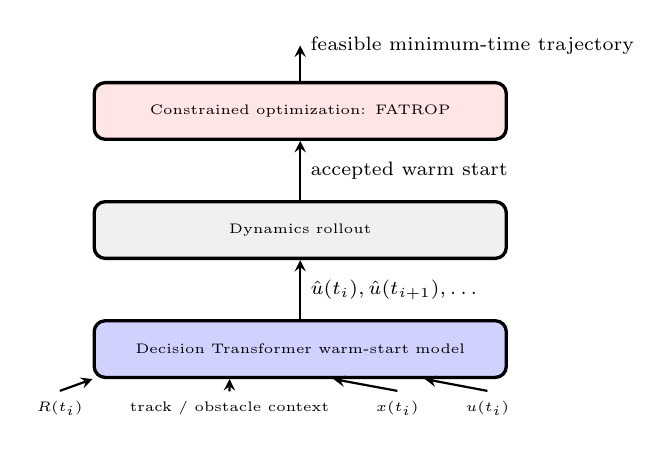
\begin{tikzpicture}[
    node distance=0.75cm,
    layer/.style={rectangle, draw, rounded corners, minimum height=0.72cm, text width=5.0cm, align=center, font=\tiny, very thick},
    token/.style={font=\tiny},
    arrow/.style={->, >=stealth, thick}
]
\node[layer, fill=red!10] (opt) {Constrained optimization: FATROP};
\node[layer, fill=gray!12, below=of opt] (dyn) {Dynamics rollout};
\node[layer, fill=blue!18, below=of dyn] (dt) {Decision Transformer warm-start model};

\node[token, below=0.15cm of dt.south west, anchor=north east] (rtg) {$R(t_i)$};
\node[token, right=0.35cm of rtg] (ctx) {track / obstacle context};
\node[token, right=0.35cm of ctx] (state) {$x(t_i)$};
\node[token, right=0.35cm of state] (act) {$u(t_i)$};
\draw[arrow] (rtg.north) -- (dt.south west);
\draw[arrow] (ctx.north) -- ($(dt.south west)!0.33!(dt.south east)$);
\draw[arrow] (state.north) -- ($(dt.south west)!0.58!(dt.south east)$);
\draw[arrow] (act.north) -- ($(dt.south west)!0.80!(dt.south east)$);

\draw[arrow] ($(dt.north)+(0,0.0)$) -- node[right, font=\scriptsize] {$\hat{u}(t_i), \hat{u}(t_{i+1}), \dots$} (dyn.south);
\draw[arrow] ($(dyn.north)+(0,0.0)$) -- node[right, font=\scriptsize, align=center] {accepted warm start} (opt.south);
\draw[arrow] ($(opt.north)+(0,0.0)$) -- ++(0,0.45) node[right, font=\scriptsize] {feasible minimum-time trajectory};
\end{tikzpicture}
\caption{Offline warm-start pipeline.}
\end{figure}
\vspace{-0.6em}
{\scriptsize
\[
\mathcal{L}_k = \|u_k-\hat{u}_k\|_2^2 + \lambda_x\|x_{k+1}^{\mathrm{obs}}-\hat{x}_{k+1}^{\mathrm{obs}}\|_2^2
\]
}
\end{column}
\begin{column}{0.46\linewidth}
\begin{itemize}
  \item Input: return-to-go, state, track, and obstacle context.
  \item Output: warm-start controls and rolled-out states.
  \item DT: context length 50, 6 layers, 4 heads, 192-dim embeddings.
  \item Loss: action imitation plus next-state consistency.
  \item Inference: autoregressive prediction with dynamics rollout.
\end{itemize}
\end{column}
\end{columns}
\end{frame}

\section{Experiments}
\begin{frame}{Experiments}
\begin{columns}[T]
\begin{column}{0.55\linewidth}
\begin{itemize}
  \item Benchmark: Oval-first evaluation with two fixed evaluation sets. The Oval track is used because it matches the setting used in the earlier Stanford GTI trajectory-optimization work:
  \begin{itemize}
    \item no-obstacle evaluation set,
    \item obstacle evaluation set with 1--4 circular obstacles.
  \end{itemize}
  \item Downstream solver: FATROP for expert generation, repair segments, and warm-started solves.
  \item Dataset mix:
  \begin{itemize}
    \item 31,710 shifted accepted full laps,
    \item 400 hard repairs,
    \item 1,000 post-projection repairs,
    \item 300 failure-conditioned repairs.
  \end{itemize}
  \item Main evaluation metrics: warm-start acceptance, fallback behavior, solver iterations, and total solve time.
\end{itemize}
\end{column}
\begin{column}{0.43\linewidth}
\begin{figure}
  \centering
  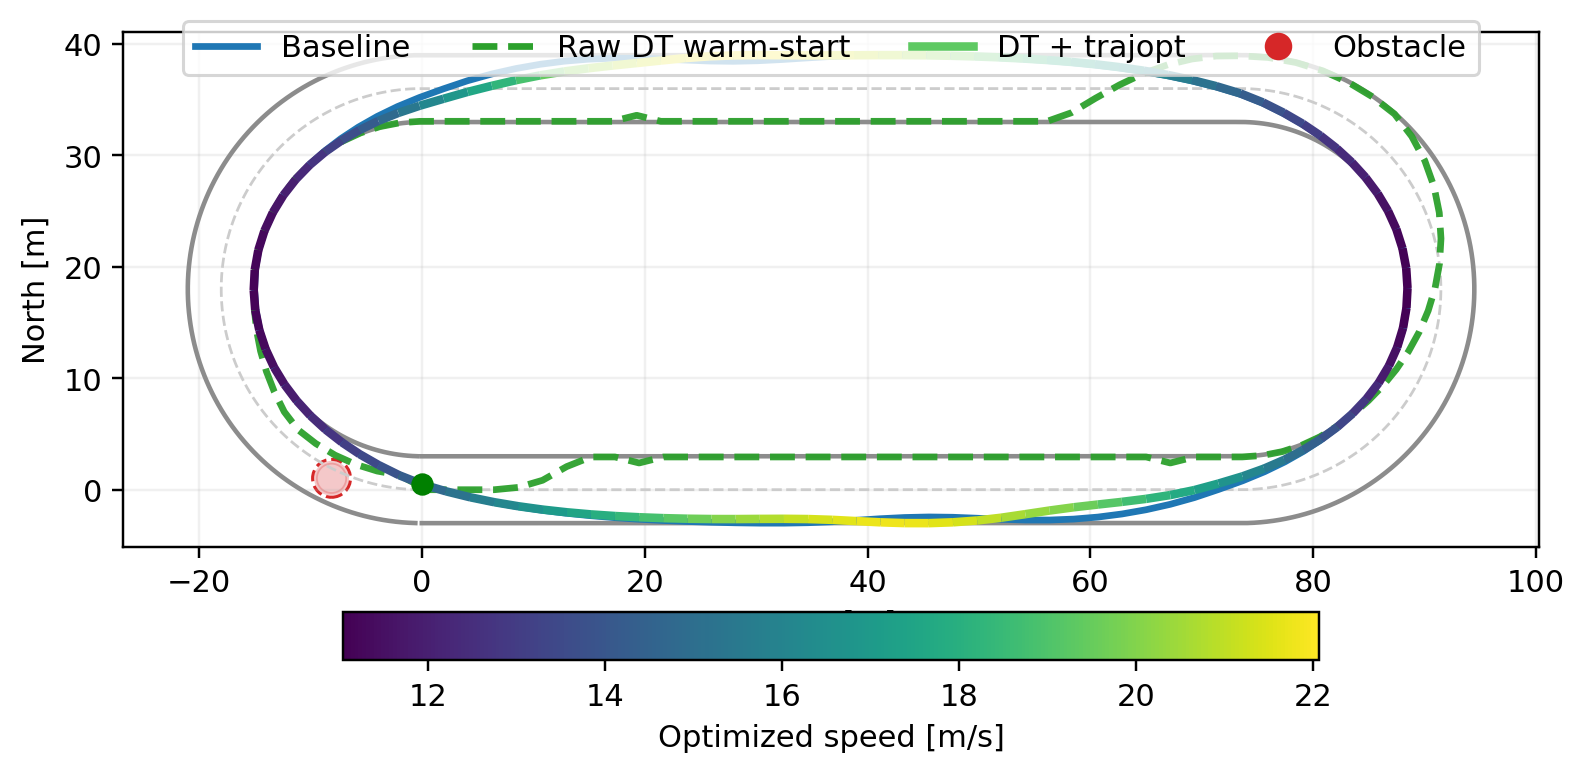
\includegraphics[width=\linewidth]{scenario000_obs3_compare.png}
  \caption{Representative obstacle case from the corrected evaluation pipeline.}
\end{figure}
\end{column}
\end{columns}
\end{frame}

\section{Trajectory Animation}
\begin{frame}{Trajectory Animation}
\begin{columns}[T]
\begin{column}{0.62\linewidth}
\begin{figure}
  \centering
  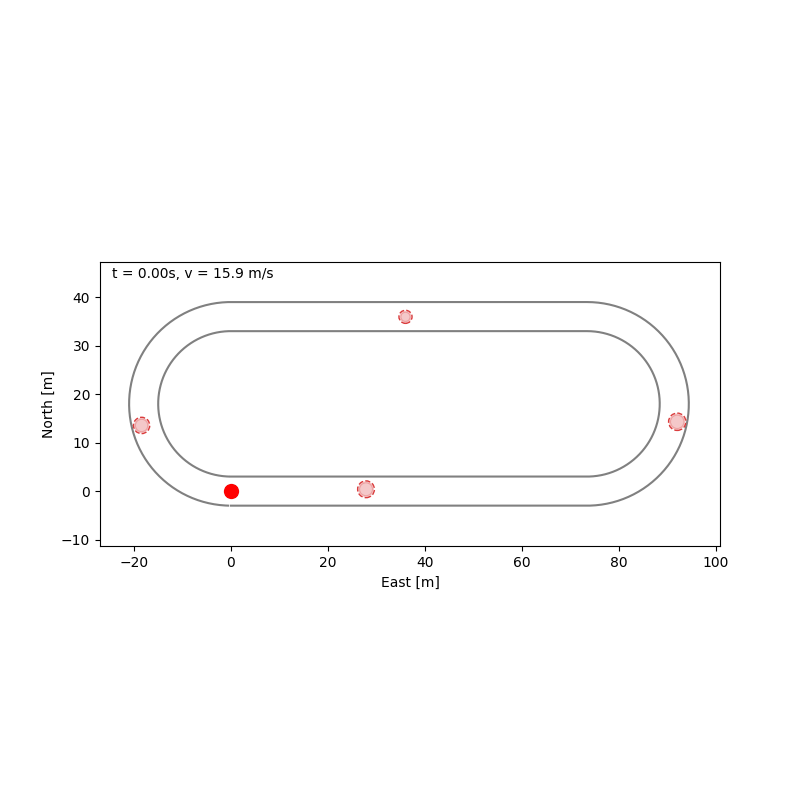
\includegraphics[width=\linewidth]{trajectory_gif_preview.png}
  \caption{Preview frame from a FATROP obstacle-track trajectory animation.}
\end{figure}
\end{column}
\begin{column}{0.34\linewidth}
\small
This slide links to the full trajectory GIF used during optimization debugging.

\vspace{0.8em}
\textbf{Asset}
\begin{itemize}
  \item FATROP obstacle-track animation
  \item Oval track with obstacles
  \item horizon $N=120$
\end{itemize}

\vspace{0.8em}
\href{run:fatrop_N120_animation.gif}{\beamerbutton{Open trajectory GIF}}

\vspace{0.8em}
% \scriptsize Works in PDF viewers that support local file links.
\end{column}
\end{columns}
\end{frame}

\section{Results and Interpretation}
\begin{frame}{Results and Interpretation}
\begin{itemize}
  \item The project started from a parent DT trained on nominal Oval trajectories and then improved the warm-start pipeline through targeted training and debugging.
  \item In later runs, raw DT trajectories became more structured, handled obstacles more plausibly, and in some cases slightly reduced solver-only time.
  \item This showed that the DT was learning useful trajectory structure, even though the full warm-start pipeline was not yet consistently faster end to end.
\end{itemize}

\vspace{0.4em}
\textbf{Main improvements during training and debugging}
\begin{itemize}
  \item larger-context DT training improved nominal trajectory quality,
  \item repair datasets exposed the model to harder rollout states,
  \item rollout and evaluation fixes made downstream behavior much easier to interpret.
\end{itemize}

\vspace{0.4em}
\begin{center}
\footnotesize
\begin{tabular}{lccc}
\toprule
\textbf{Setting} & \textbf{WS accept} & \textbf{Baseline solve} & \textbf{DT total} \\
\midrule
No obstacles & 20\% & 49.06s & 51.98s \\
1--4 obstacles & 20\% & 56.36s & 60.79s \\
\bottomrule
\end{tabular}
\end{center}
\end{frame}

\begin{frame}{Results: Training and Qualitative Behavior}
\begin{columns}[T]
\begin{column}{0.48\linewidth}
\begin{figure}
  \centering
  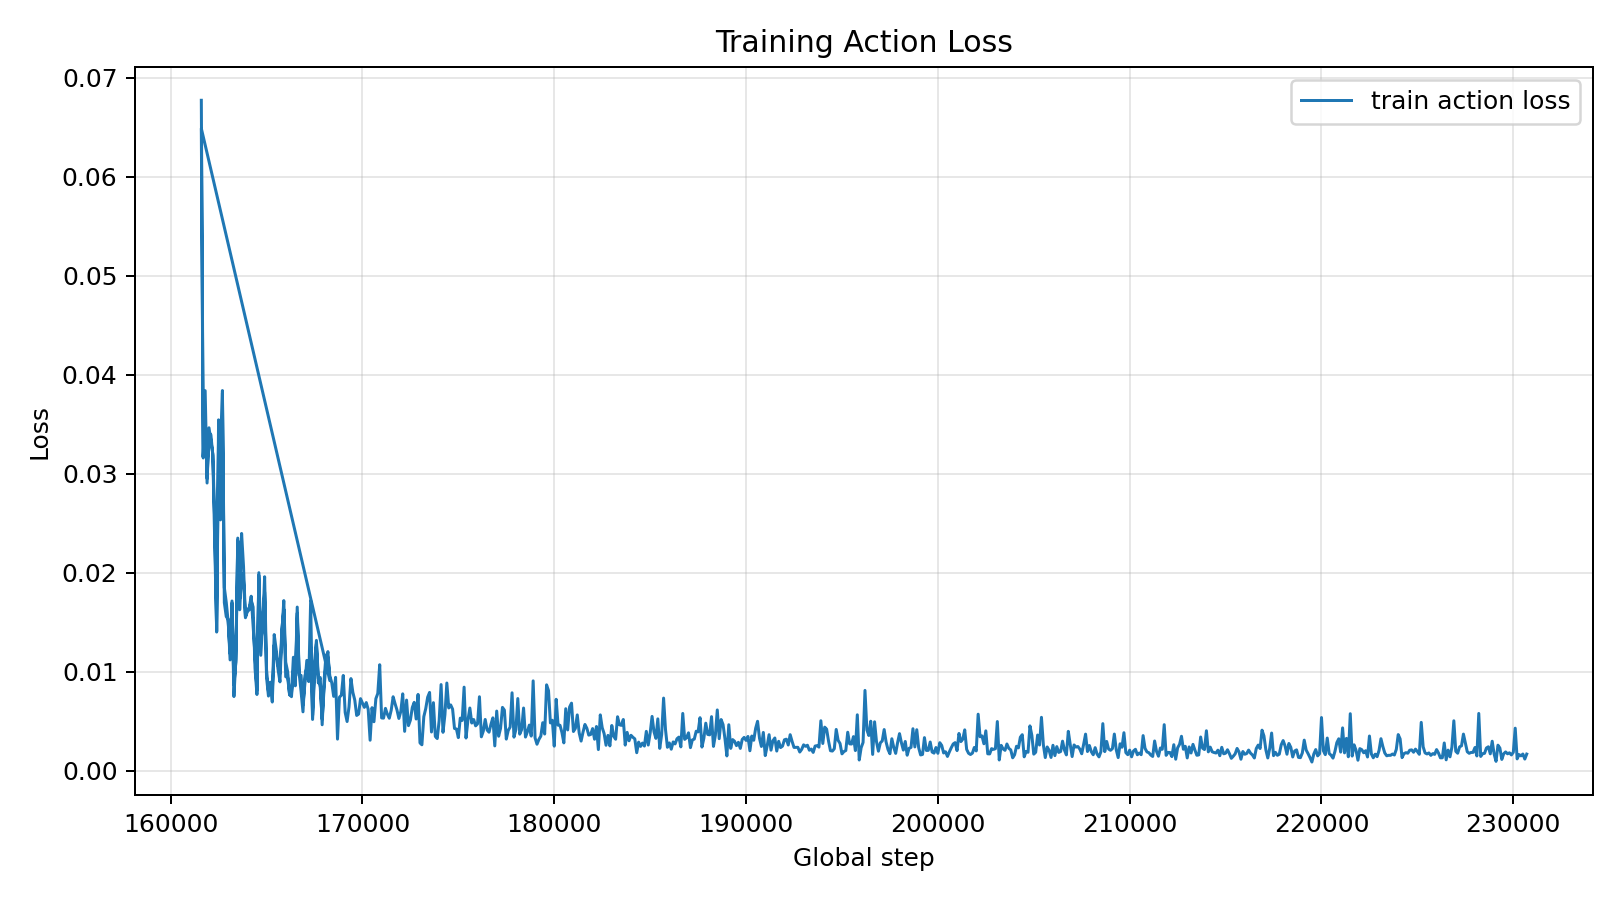
\includegraphics[width=0.9\linewidth]{postproj_ft2_train_loss_curves.png}
  \caption{Later fine-tuning runs trained stably under the larger-context DT setup.}
\end{figure}
\end{column}
\begin{column}{0.48\linewidth}
\begin{itemize}
  \item The strongest result was not a full end-to-end speedup, but a more interpretable and more structured warm-start behavior.
  \item Across stricter evaluation settings, the same pattern remained:
  \begin{itemize}
    \item plausible raw DT trajectories,
    \item occasional solver-only benefit,
    \item but not yet reliable end-to-end gains.
  \end{itemize}
  \item A major project outcome was identifying the remaining bottleneck clearly enough to target the next iteration.
\end{itemize}
\end{column}
\end{columns}
\end{frame}

\section{Conclusions and Next Steps}
\begin{frame}{Conclusions and Next Steps}
\begin{itemize}
  \item The main contribution is a working framework for learned warm-starts in constrained racing trajectory optimization.
  \item The full pipeline now covers:
  \begin{itemize}
    \item offline expert generation,
    \item DT training and fine-tuning,
    \item repair-data generation,
    \item rollout diagnostics,
    \item downstream benchmarking.
  \end{itemize}
  \item The DT learned meaningful trajectory structure and produced real warm-start signal.
  \item The harder lesson was that deployment metrics matter more than offline loss alone.
\end{itemize}

\vspace{0.5em}
\textbf{Next step:} continue training on the difficult rollout states revealed by diagnostics so that improved raw DT trajectory quality turns into more consistent optimizer gains.
\end{frame}

\section{References}
\begin{frame}{References}
\footnotesize
\begin{enumerate}
  \item J. K. Subosits and J. C. Gerdes, ``Impacts of Model Fidelity on Trajectory Optimization for Autonomous Vehicles in Extreme Maneuvers,'' \textit{IEEE Transactions on Intelligent Vehicles}, 2021.
  \item L. Chen et al., ``Decision Transformer: Reinforcement Learning via Sequence Modeling,'' \textit{Advances in Neural Information Processing Systems}, 2021.
  \item T. Guffanti and S. D'Amico, ``Transformers for Trajectory Optimization with Application to Spacecraft Rendezvous,'' \textit{IEEE Aerospace Conference}, 2024.
\end{enumerate}
\end{frame}

\end{document}
